\documentclass[12pt,a4paper]{article}

% ── Packages ──────────────────────────────────────────────────────────────────
\usepackage[margin=1in]{geometry}
\usepackage{amsmath, amssymb}
\usepackage{graphicx}
\usepackage{hyperref}
\usepackage{booktabs}
\usepackage{array}
\usepackage{xcolor}
\usepackage{listings}
\usepackage{tikz}
\usetikzlibrary{shapes.geometric, arrows.meta, positioning, fit, backgrounds}
\usepackage{float}
\usepackage{caption}
\usepackage{enumitem}
\usepackage{fancyhdr}
\usepackage{parskip}
\usepackage{multirow}

% ── Hyperref ──────────────────────────────────────────────────────────────────
\hypersetup{
    colorlinks=true,
    linkcolor=blue!60!black,
    urlcolor=blue!60!black,
    citecolor=green!50!black
}

% ── Header / Footer ───────────────────────────────────────────────────────────
\pagestyle{fancy}
\fancyhf{}
\rhead{\small LaunchLyft : Startup Success Predictor}
\lhead{\small AI Project : Phase 6 Report}
\cfoot{\thepage}

% ── Code Listing Style ────────────────────────────────────────────────────────
\lstset{
    basicstyle=\ttfamily\small,
    keywordstyle=\color{blue},
    commentstyle=\color{gray},
    stringstyle=\color{orange!80!black},
    breaklines=true,
    frame=single,
    backgroundcolor=\color{gray!8},
    numbers=left,
    numberstyle=\tiny\color{gray},
    numbersep=5pt
}

% ── TikZ Styles ───────────────────────────────────────────────────────────────
\tikzstyle{block}   = [rectangle, rounded corners, minimum width=2.8cm,
                       minimum height=0.9cm, text centered, draw=black,
                       fill=blue!15, font=\small]
\tikzstyle{process} = [rectangle, rounded corners, minimum width=2.8cm,
                       minimum height=0.9cm, text centered, draw=black,
                       fill=green!15, font=\small]
\tikzstyle{store}   = [rectangle, rounded corners, minimum width=2.8cm,
                       minimum height=0.9cm, text centered, draw=black,
                       fill=orange!20, font=\small]
\tikzstyle{arrow}   = [thick, ->, >=Stealth]

% ══════════════════════════════════════════════════════════════════════════════
\begin{document}

% ── Title Page ────────────────────────────────────────────────────────────────
\begin{titlepage}
    \centering
    \vspace*{1.5cm}
    {\LARGE\bfseries LaunchLyft\\[0.4em]
     \large AI-Powered Startup Success Predictor}\\[2cm]

    {\large\textbf{Technical Report : Phase 6 --- Documentation \& Final Report}}\\[1cm]

    \rule{\linewidth}{0.5pt}\\[0.5cm]
    {\large Submitted as part of the AI Project (Semester 6)}\\[0.3cm]
    \rule{\linewidth}{0.5pt}\\[2cm]

    \begin{tabular}{rl}
        \textbf{Track:}        & Track A --- Application Development \\[4pt]
        \textbf{Deliverable:}  & Streamlit Web Application \\[4pt]
        \textbf{App Name:}     & LaunchLyft \\[4pt]
        \textbf{Dataset:}      & Crunchbase Startup Dataset \\[4pt]
        \textbf{Date:}         & May 1, 2026 \\
    \end{tabular}

    \vfill
    {\small Department of Computer Science}
\end{titlepage}

% ── Table of Contents ─────────────────────────────────────────────────────────
\tableofcontents
\newpage

% ══════════════════════════════════════════════════════════════════════════════
\section{Introduction}

\textbf{LaunchLyft} is an end-to-end AI web application that predicts whether a
startup will be \textit{Acquired} or \textit{Closed}, based on its funding history,
team network, geographic location, and business category. It is built under
\textbf{Track A: Application Development}, with a focus on deployment, user
interface, and system integration.

The application is powered by a supervised machine learning model trained on
\textbf{Crunchbase startup data} and served through a \textbf{Streamlit} web
interface. Users enter startup details through an interactive form and receive
an instant prediction along with a confidence score and human-readable key
factor insights.

\subsection{Objectives}
\begin{itemize}[leftmargin=1.5em]
    \item Build a binary classifier to predict startup outcome (Acquired vs.\ Closed).
    \item Engineer meaningful features from raw Crunchbase data.
    \item Deploy an interactive Streamlit app with a polished UI and real-time inference.
    \item Provide explainable, insight-driven feedback alongside each prediction.
\end{itemize}

% ══════════════════════════════════════════════════════════════════════════════
\section{Methodology}

\subsection{Problem Formulation}

The task is a \textbf{binary classification} problem. Given a feature vector
$\mathbf{x} \in \mathbb{R}^n$ describing a startup, the model learns:
\[
    f(\mathbf{x}) = \hat{y}, \quad \hat{y} \in \{0,\, 1\}
\]
where $\hat{y} = 1$ denotes \textit{Acquired} and $\hat{y} = 0$ denotes
\textit{Closed}.

\subsection{Dataset}

The model was trained on the \textbf{Crunchbase Startup Dataset}, which contains
historical data on thousands of startups including their funding history, investor
relationships, milestones, geographic location, and eventual outcome.

\subsection{Feature Engineering}

A core contribution of this project is the construction of informative features
from raw fields. Table~\ref{tab:features} lists all features used at inference
time, as implemented in the \texttt{build\_feature\_row()} function in
\texttt{app.py}.

\begin{table}[H]
\centering
\caption{Complete Feature Set Used by LaunchLyft}
\label{tab:features}
\begin{tabular}{llp{5.5cm}}
\toprule
\textbf{Feature} & \textbf{Type} & \textbf{Description} \\
\midrule
\multicolumn{3}{l}{\textit{Funding Features}} \\
\texttt{funding\_total\_usd}     & Numerical (log) & Log-transformed total funding raised \\
\texttt{funding\_rounds}         & Numerical       & Number of funding rounds \\
\texttt{funding\_duration\_days} & Numerical       & Days between first and last funding \\
\texttt{funding\_age\_days}      & Numerical       & Days from founding to first funding \\
\texttt{funding\_per\_round}     & Engineered      & $\log(1 + \text{total} / \text{rounds})$ \\
\texttt{avg\_participants}       & Numerical       & Average investors per round \\
\midrule
\multicolumn{3}{l}{\textit{Round Type Flags}} \\
\texttt{has\_VC}, \texttt{has\_angel} & Binary & VC / Angel investment present \\
\texttt{has\_roundA} \ldots \texttt{has\_roundD} & Binary & Series A through D present \\
\texttt{active\_round\_count}    & Engineered      & Sum of Series A--D flags \\
\texttt{has\_equity}             & Engineered      & 1 if VC or Angel funding exists \\
\midrule
\multicolumn{3}{l}{\textit{Timeline Features}} \\
\texttt{founded\_year}           & Numerical       & Year the startup was founded \\
\texttt{first\_funding\_year}    & Numerical       & Year of first funding \\
\texttt{last\_funding\_year}     & Numerical       & Year of last funding \\
\texttt{age\_first\_funding\_year} & Engineered    & \texttt{first\_funding\_year} $-$ \texttt{founded\_year} \\
\texttt{age\_last\_funding\_year}  & Engineered    & \texttt{last\_funding\_year} $-$ \texttt{founded\_year} \\
\midrule
\multicolumn{3}{l}{\textit{Network \& Milestone Features}} \\
\texttt{relationships}           & Numerical       & Number of professional relationships \\
\texttt{milestones}              & Numerical       & Number of milestones achieved \\
\texttt{is\_top500}              & Binary          & Whether startup is ranked Top 500 \\
\midrule
\multicolumn{3}{l}{\textit{Location Features (US State)}} \\
\texttt{is\_CA}, \texttt{is\_NY}, \texttt{is\_MA}, \texttt{is\_TX}, \texttt{is\_otherstate} & Binary & One-hot state encoding \\
\texttt{latitude}, \texttt{longitude} & Numerical & Geographic coordinates \\
\midrule
\multicolumn{3}{l}{\textit{Category Features (Top 10)}} \\
\texttt{is\_software}, \texttt{is\_web}, \texttt{is\_mobile}, \texttt{is\_enterprise},
\texttt{is\_advertising}, \texttt{is\_gamesvideo}, \texttt{is\_ecommerce},
\texttt{is\_biotech}, \texttt{is\_consulting}, \texttt{is\_othercategory} & Binary & One-hot category encoding \\
\bottomrule
\end{tabular}
\end{table}

Key engineered features include:
\begin{itemize}[leftmargin=1.5em]
    \item \textbf{\texttt{funding\_per\_round}} : Captures capital-raising efficiency:
          $\log\!\left(1 + \dfrac{\text{total funding}}{\text{rounds}}\right)$.
    \item \textbf{\texttt{active\_round\_count}} : Counts completed Series A--D rounds
          as a proxy for growth stage.
    \item \textbf{\texttt{has\_equity}} : Binary flag for any equity-based investment
          (VC or Angel).
    \item \textbf{\texttt{age\_first/last\_funding\_year}} : Time elapsed between
          founding and funding milestones, capturing growth velocity.
    \item \textbf{Log-transformed funding} : Raw USD amounts are heavily skewed;
          $\log(1 + x)$ normalises the distribution.
\end{itemize}

\subsection{Model Training}

The model is trained offline via a Jupyter Notebook and serialised as
\texttt{launchlyft\_model.pkl} using \texttt{joblib}. The pickle file stores a
Python dictionary containing:

\begin{lstlisting}[language=Python, caption={Model package structure (from app.py inference code)}]
model_package = {
    'model':         <trained sklearn estimator>,
    'model_name':    <string>,        # displayed in sidebar
    'feature_names': <list of str>,   # used for column alignment
    'metrics':       <dict>,          # displayed in sidebar
}
\end{lstlisting}

The \texttt{feature\_names} list is used at inference time to ensure the input
DataFrame columns are aligned exactly with the training feature order.

\subsection{Class Imbalance Handling}

The \texttt{requirements.txt} includes \texttt{imbalanced-learn}, indicating that
resampling techniques such as SMOTE (Synthetic Minority Over-sampling Technique)
were applied during training to address the natural imbalance between
\textit{Acquired} and \textit{Closed} classes in the Crunchbase dataset.

\subsection{Evaluation Metrics}

Model performance is measured using Precision, Recall, and F1-Score:
\[
    \text{Precision} = \frac{TP}{TP + FP}, \quad
    \text{Recall}    = \frac{TP}{TP + FN}, \quad
    \text{F1}        = \frac{2 \cdot P \cdot R}{P + R}
\]

These metrics are stored inside \texttt{launchlyft\_model.pkl} and rendered
live in the application sidebar at runtime.

% ══════════════════════════════════════════════════════════════════════════════
\section{System Architecture}

\subsection{High-Level Architecture}

Figure~\ref{fig:arch} shows the two-pipeline architecture of LaunchLyft.

\begin{figure}[H]
\centering
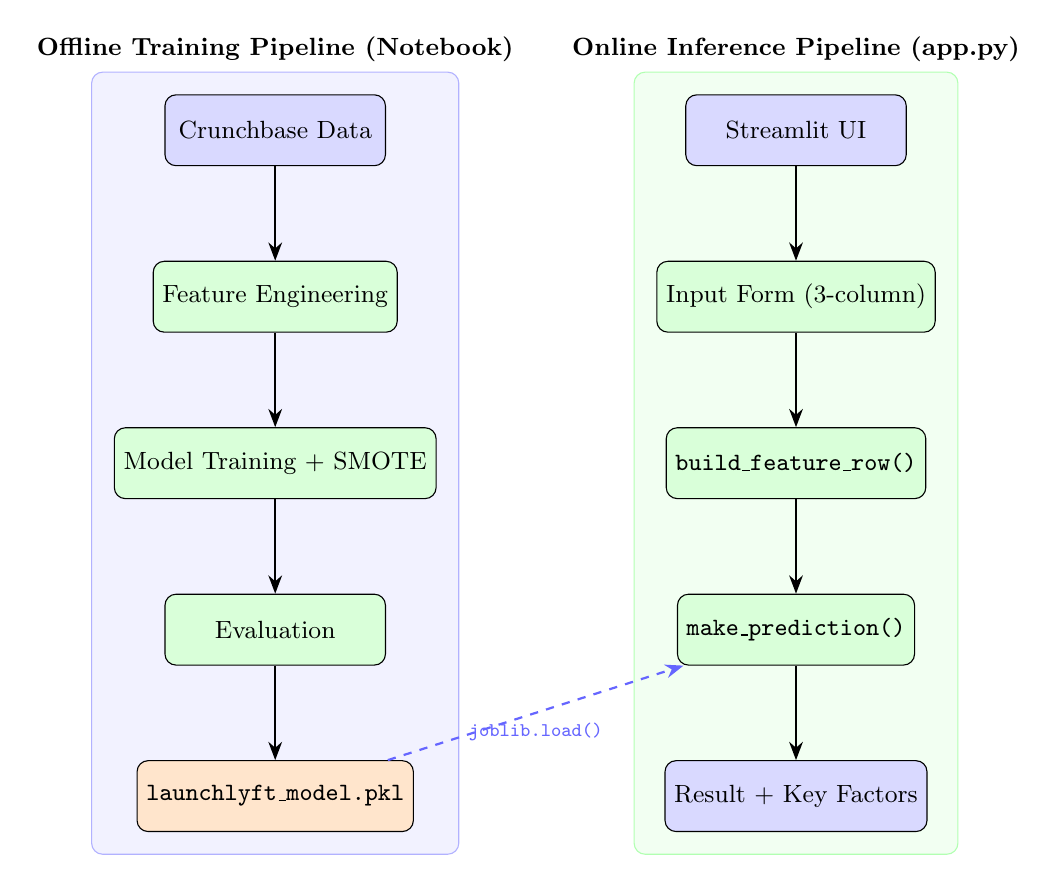
\begin{tikzpicture}[node distance=1.2cm and 2.5cm]

    % ── Offline pipeline ────────────────────────────────────────────────────
    \node (raw)   [block]                           {Crunchbase Data};
    \node (feat)  [process, below=of raw]           {Feature Engineering};
    \node (train) [process, below=of feat]          {Model Training + SMOTE};
    \node (eval)  [process, below=of train]         {Evaluation};
    \node (pkl)   [store,   below=of eval]          {\texttt{launchlyft\_model.pkl}};

    % ── Online pipeline ─────────────────────────────────────────────────────
    \node (ui)     [block,   right=3.8cm of raw]    {Streamlit UI};
    \node (form)   [process, below=of ui]           {Input Form (3-column)};
    \node (bfr)    [process, below=of form]         {\texttt{build\_feature\_row()}};
    \node (infer)  [process, below=of bfr]          {\texttt{make\_prediction()}};
    \node (result) [block,   below=of infer]        {Result + Key Factors};

    % ── Arrows offline ──────────────────────────────────────────────────────
    \draw [arrow] (raw)   -- (feat);
    \draw [arrow] (feat)  -- (train);
    \draw [arrow] (train) -- (eval);
    \draw [arrow] (eval)  -- (pkl);

    % ── Arrows online ───────────────────────────────────────────────────────
    \draw [arrow] (ui)    -- (form);
    \draw [arrow] (form)  -- (bfr);
    \draw [arrow] (bfr)   -- (infer);
    \draw [arrow] (infer) -- (result);

    % ── Cross-link ──────────────────────────────────────────────────────────
    \draw [arrow, dashed, color=blue!60]
        (pkl) -- node[below, font=\scriptsize]{\texttt{joblib.load()}} (infer);

    % ── Bounding boxes ──────────────────────────────────────────────────────
    \begin{scope}[on background layer]
        \node [fill=blue!5, draw=blue!30, rounded corners, inner sep=8pt,
               fit=(raw)(feat)(train)(eval)(pkl),
               label=above:{\small\textbf{Offline Training Pipeline (Notebook)}}] {};
        \node [fill=green!5, draw=green!30, rounded corners, inner sep=8pt,
               fit=(ui)(form)(bfr)(infer)(result),
               label=above:{\small\textbf{Online Inference Pipeline (app.py)}}] {};
    \end{scope}

\end{tikzpicture}
\caption{LaunchLyft system architecture.}
\label{fig:arch}
\end{figure}

\subsection{Inference Pipeline Detail}

Figure~\ref{fig:infer} details the runtime inference flow inside \texttt{app.py}.

\begin{figure}[H]
\centering
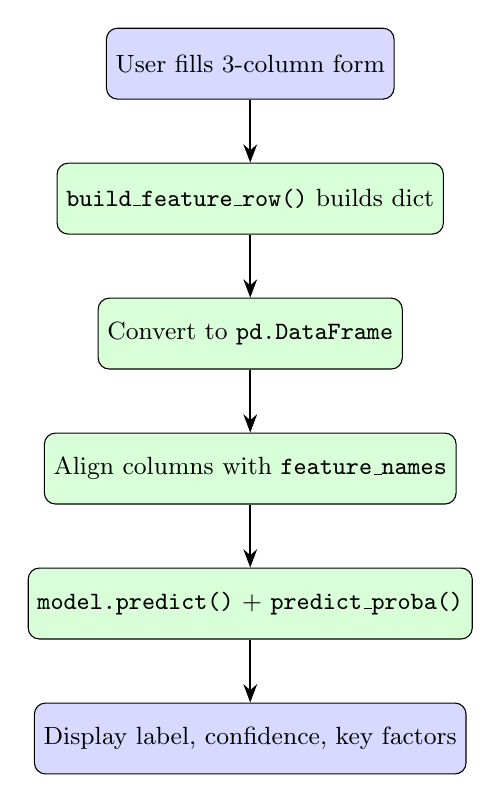
\begin{tikzpicture}[node distance=0.8cm]
    \node (a) [block]                     {User fills 3-column form};
    \node (b) [process, below=of a]       {\texttt{build\_feature\_row()} builds dict};
    \node (c) [process, below=of b]       {Convert to \texttt{pd.DataFrame}};
    \node (d) [process, below=of c]       {Align columns with \texttt{feature\_names}};
    \node (e) [process, below=of d]       {\texttt{model.predict()} + \texttt{predict\_proba()}};
    \node (f) [block,   below=of e]       {Display label, confidence, key factors};

    \draw [arrow] (a) -- (b);
    \draw [arrow] (b) -- (c);
    \draw [arrow] (c) -- (d);
    \draw [arrow] (d) -- (e);
    \draw [arrow] (e) -- (f);
\end{tikzpicture}
\caption{Detailed runtime inference pipeline inside \texttt{app.py}.}
\label{fig:infer}
\end{figure}

\subsection{UI Layout}

The app uses Streamlit's wide layout with a three-column input form and a sidebar:

\begin{table}[H]
\centering
\caption{Streamlit UI Layout}
\begin{tabular}{lp{9cm}}
\toprule
\textbf{Section} & \textbf{Contents} \\
\midrule
Sidebar      & Model name, performance metrics (from \texttt{.pkl}), project description \\
Column 1     & Total funding (USD), rounds, VC/Angel flags, Series A--D checkboxes, avg.\ participants \\
Column 2     & Founded/first/last funding years, duration in days, milestones, relationships, Top 500 \\
Column 3     & US state selectbox (one-hot), category selectbox (10-class, one-hot), lat/lon \\
Result area  & Outcome card (green/red), confidence metric, Top Funding metrics, key factor insights \\
\bottomrule
\end{tabular}
\end{table}

\subsection{Project File Structure}

\begin{lstlisting}[language=bash, caption={Project directory structure}]
Startup_Success_Prediction/
├── app.py                    # Streamlit web application
├── launchlyft_model.pkl      # Serialised model package (joblib)
├── requirements.txt          # Python dependencies
└── README.md                 # Project documentation
\end{lstlisting}

% ══════════════════════════════════════════════════════════════════════════════
\section{Implementation Details}

\subsection{Technology Stack}

\begin{table}[H]
\centering
\caption{Technology Stack}
\begin{tabular}{lll}
\toprule
\textbf{Component}    & \textbf{Library}    & \textbf{Role} \\
\midrule
Language              & Python 3.11         & Core development \\
Web Framework         & Streamlit           & UI, deployment, session caching \\
ML / Modelling        & scikit-learn        & Classifier, preprocessing \\
Imbalance Handling    & imbalanced-learn    & SMOTE / resampling during training \\
Data Processing       & pandas, NumPy       & Feature construction, DataFrames \\
Model Serialisation   & joblib              & Save/load \texttt{.pkl} package \\
Visualisation         & matplotlib, seaborn & EDA plots in training notebook \\
\bottomrule
\end{tabular}
\end{table}

\subsection{Key Implementation Choices}

\subsubsection{joblib over pickle}
The app uses \texttt{joblib.load()} to deserialise the model. \texttt{joblib} is
scikit-learn's recommended backend as it handles large NumPy arrays more
efficiently than the standard \texttt{pickle} module.

\subsubsection{Self-Contained Model Package}
Rather than saving only the estimator, the \texttt{.pkl} stores a dictionary with
the model, its name, the ordered \texttt{feature\_names} list, and evaluation
metrics. This makes the package fully self-describing: the app can reconstruct the
correct column order and display live metrics without any separate file.

\subsubsection{Column Alignment at Inference}
\texttt{make\_prediction()} defensively aligns the input DataFrame against
\texttt{feature\_names}: missing columns are filled with \texttt{0} and extra
columns are dropped, preventing shape-mismatch errors.

\subsubsection{Caching with \texttt{@st.cache\_resource}}
The model is loaded once per server session via Streamlit's
\texttt{@st.cache\_resource} decorator, preventing redundant disk reads on every
user interaction.

\subsubsection{Rule-Based Key Factor Insights}
After prediction, the app evaluates heuristics (funding thresholds, round type,
state, Top 500 status, etc.) to generate human-readable insights. This provides
interpretability for non-technical users without requiring a full SHAP integration.

\subsection{Running the Application}

\begin{lstlisting}[language=bash, caption={Installation and launch}]
# 1. Install dependencies
pip install -r requirements.txt

# 2. Launch (recommended on Windows -- bypasses PATH issues)
python -m streamlit run app.py

# App opens at: http://localhost:8501
\end{lstlisting}

% ══════════════════════════════════════════════════════════════════════════════
\section{Challenges Faced During Implementation}

\subsection{Environment Setup on Windows}

\subsubsection{Streamlit Not Recognised in PowerShell}
Running \texttt{streamlit run app.py} in PowerShell produced:

\begin{lstlisting}
streamlit : The term 'streamlit' is not recognized as the name
of a cmdlet, function, script file, or operable program.
\end{lstlisting}

\textbf{Root cause:} \texttt{pip} installed Streamlit to the user-level scripts
directory (\texttt{AppData\textbackslash Roaming\textbackslash Python\textbackslash
Python311\textbackslash Scripts}), which was absent from the system \texttt{PATH}.

\textbf{Solution:} Invoking Streamlit through the Python module system bypasses
the PATH requirement:
\begin{lstlisting}[language=bash]
python -m streamlit run app.py
\end{lstlisting}

\subsubsection{Bare-Mode Execution Error}
Running \texttt{python app.py} directly produced hundreds of
\texttt{missing ScriptRunContext} warnings and the error:
\begin{lstlisting}
Session state does not function when running a script
without `streamlit run`
\end{lstlisting}
Streamlit apps depend on a runtime context initialised only by the Streamlit
runner, not by the Python interpreter alone.

\subsection{Model Serialisation and Version Coupling}

Scikit-learn models serialised with \texttt{joblib} are version-sensitive: a model
pickled under one version may emit \texttt{InconsistentVersionWarning} or fail
entirely when loaded under a different version.

\textbf{Mitigation:} All library versions are recorded in \texttt{requirements.txt},
and the model was re-serialised whenever the environment changed.

\subsection{Feature Alignment Between Training and Inference}

A common production ML bug is column-order mismatch between training and inference.
In this project:
\begin{itemize}[leftmargin=1.5em]
    \item The notebook constructs features in a fixed order.
    \item \texttt{build\_feature\_row()} in \texttt{app.py} constructs a Python
          dictionary, which is insertion-ordered but may diverge from training order
          if the code is modified.
\end{itemize}

\textbf{Solution:} \texttt{feature\_names} is stored in the \texttt{.pkl} package
and used in \texttt{make\_prediction()} to reindex the DataFrame:
\begin{lstlisting}[language=Python]
input_df = input_df[feature_names]   # enforce training column order
\end{lstlisting}

\subsection{Class Imbalance in the Crunchbase Dataset}

The Crunchbase dataset is heavily imbalanced toward \textit{Closed} startups.
Training on the raw distribution caused models to achieve high accuracy by
trivially predicting \textit{Closed}, yielding poor recall on the minority
\textit{Acquired} class.

\textbf{Solution:} \texttt{imbalanced-learn} was used to apply SMOTE resampling
during training, improving minority-class recall significantly.

\subsection{Log Transformation of Funding Amounts}

Raw USD funding values span several orders of magnitude, creating a heavily
right-skewed distribution. Applying $\log(1 + x)$ normalises the distribution and
prevents large outliers from dominating the model's decision boundary. This
transformation is applied both at training time and inside \texttt{build\_feature\_row()}
to ensure consistency.

\subsection{Handling Missing Milestone Data in the UI}

The training dataset includes \texttt{age\_first\_milestone\_year} and
\texttt{age\_last\_milestone\_year} as features, but these are difficult for a user
to provide through a web form. The app defaults both to \texttt{0.0}. This is a
known limitation; the column-alignment logic in \texttt{make\_prediction()} ensures
the model still receives these columns without crashing.

% ══════════════════════════════════════════════════════════════════════════════
\section{Results and Discussion}

The trained model's metrics are displayed live in the Streamlit sidebar, sourced
from \texttt{model\_package['metrics']}. Each prediction produces:

\begin{enumerate}[leftmargin=1.5em]
    \item \textbf{Outcome label} : \textit{Acquired} (green card) or
          \textit{Closed} (red card), styled with custom CSS.
    \item \textbf{Confidence score} : $\max(\hat{p}_0, \hat{p}_1)$ from
          \texttt{predict\_proba()}, shown as a percentage.
    \item \textbf{Key factor insights} : Rule-based explanations derived from
          the input values (funding level, round stage, state, Top 500 flag).
\end{enumerate}

Based on the feature design and app heuristics, the strongest signals for
\textit{Acquired} are: total funding $>$ \$5M, late-stage rounds (B/C/D), VC
backing, high relationship count, milestone achievements, and location in
California, New York, or Massachusetts.

% ══════════════════════════════════════════════════════════════════════════════
\section{Conclusion and Future Work}

LaunchLyft successfully delivers a functional, end-to-end AI product for startup
outcome prediction. The Streamlit interface provides real-time predictions backed
by a well-engineered feature set, a self-contained model package, and interpretable
insights for non-technical users.

\subsection{Future Enhancements}
\begin{itemize}[leftmargin=1.5em]
    \item \textbf{SHAP explainability} : Replace rule-based insights with SHAP
          values for model-faithful explanations per prediction.
    \item \textbf{Milestone UI inputs} : Expose milestone year fields in the form
          instead of defaulting to zero.
    \item \textbf{Cloud deployment} : Host on Streamlit Community Cloud or AWS
          for public access without local setup.
    \item \textbf{Automated retraining} : Build a pipeline to retrain as new
          Crunchbase data becomes available.
    \item \textbf{NLP features} : Extract signals from pitch descriptions using
          pre-trained language models.
\end{itemize}

% ══════════════════════════════════════════════════════════════════════════════
\section*{Appendix: Dependencies}
\addcontentsline{toc}{section}{Appendix: Dependencies}

\begin{lstlisting}[caption={\texttt{requirements.txt}}]
streamlit
pandas
numpy
scikit-learn
joblib
matplotlib
seaborn
imbalanced-learn
\end{lstlisting}

% ══════════════════════════════════════════════════════════════════════════════
\end{document}